\section{Proposed Work}

\begin{figure}[h]
    \centering
    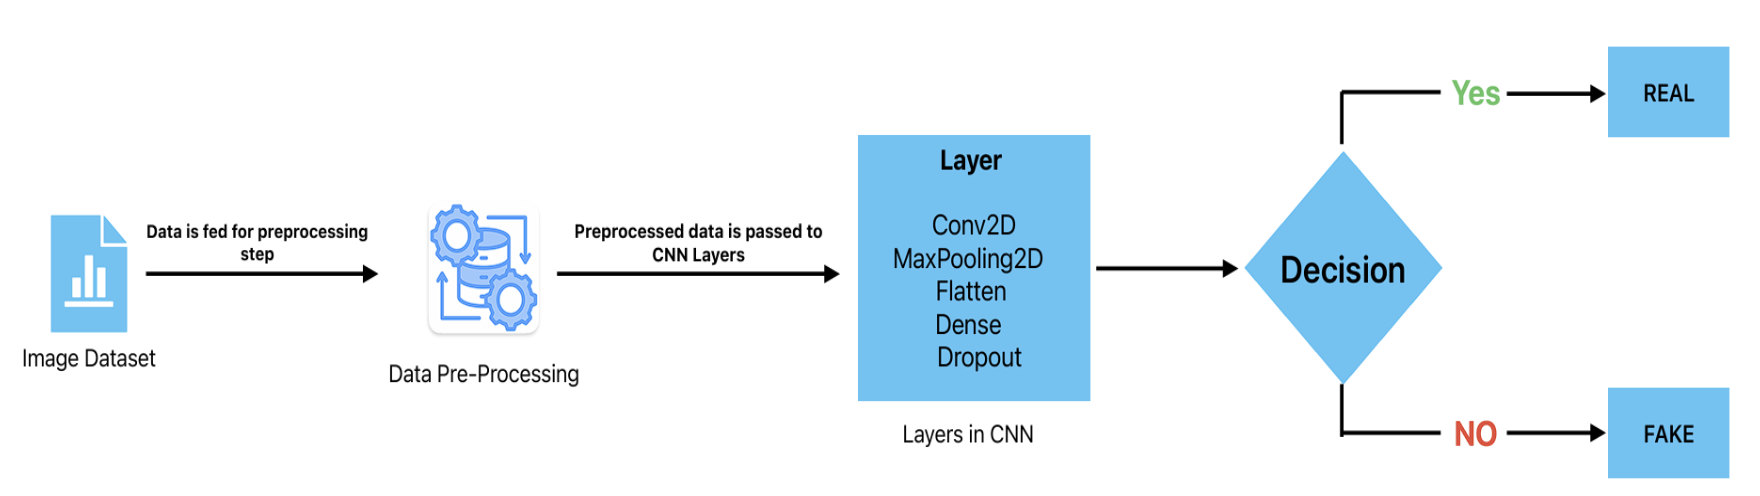
\includegraphics[width=1\textwidth]{figures/proposed_model.png}
    \caption{Proposed Model}
    \label{fig:enter-label}
\end{figure}

\subsection{Model Architecture}

The CNN model consists of three convolutional layers followed by max pooling layers to
extract features from the images. The convolutional layers use ReLU activation functions
to introduce non-linearity, and the max pooling layers reduce the spatial dimensions of
the feature maps. A flatten layer is used to convert the 2D feature maps into a 1D vector,
which is then passed through two dense layers with ReLU activation functions
\subsection{Model Training}

The model is compiled using the Adam optimizer and binary cross-entropy loss
function, as it is a binary classification problem. The model is trained for 10epochs using the augmented training data. During training, the fit method is called on the model, passing the augmented training data generator and the
validation data.The steps per epoch parameter is set to the number of training samples divided by the batch size.
\subsection{Model Evaluation}
After training, the model is evaluated using the testing set. The evaluate
method is called on the model, passing the testing data, and the loss and
accuracy metrics are computed. Additionally, the model is used to make
predictions on the testing set, and the predictions are compared against the
ground truth labels to calculate the confusion matrix, accuracy, recall, and
precision scores.
\subsection{Prediction}

Finally, the trained model is used to make predictions on a sample image. The
image is loaded and preprocessed using the same steps as the training
images. The model's predict method is called on the preprocessed image, and
the output probability is used to classify the image as real or fake.
Overall, the deep fake detection system leverages CNNs and data
augmentation to accurately detect manipulated images, contributing to the
ongoing efforts to combat the spread of misinformation and protect the integrity of digital media







